\begin{savequote}[45mm]
\ascii{Any fool can write code that a computer can understand. Good programmers write code that humans can understand.}
\qauthor{\ascii{- Martin Flower}}
\end{savequote}

\chapter{聚集参数} 
\label{ch:param-collector}

\begin{content}

本章重点讨论收集测试结果的实现机制,重构趋向\emph{聚集参数}模式。聚集参数由\ascii{Kent Beck}在其经典著作《实现模式》中引入的,他将\emph{聚集参数}抽象为一个对象,并传递给不同的函数,以便在函数调用链中聚集结果。

\end{content}

\section{收集器}

\begin{content}

在之前的测试用例中,为了统计测试用例的运行数目,在匿名命名空间内引入计数器\ascii{num}。当某个用例被执行时,执行计数器的累加操作。显而易见,计数器游离在对象之外是极为危险的,即使该计数器已经被限制在匿名命名空间内。因为,在其可见的作用域内都有可能被他人修改。

这是一种脆弱的设计,用户需要小心地维护计数器的初始化,及其精细控制计数器累加的时机。其一,容易引入未初始化的错误。其二,使得操作计数器的代码散乱到各个子类覆写的\ascii{runTest}之中,违背了高内聚的基本设计原则。其三,客户承担的职责过多,并产生重复的客户代码。

\begin{nodiff}{test/mars/core/TestSuiteSpec.cc}
 \begin{c++}
#include <mars/core/TestSuite.h>
#include <mars/core/TestCase.h>
#include <gtest/gtest.h>

namespace {
@  int num = 0;@

  struct FooTest : TestCase {
  private:
    void runTest() override {
@      num++;@
    }
  };

  struct TestSuiteSpec : testing::Test {
  private:
    void SetUp() override {
@      num = 0;@
    }
  };
}

TEST_F(TestSuiteSpec, pack_test_cases_into_test_suite) {
  TestSuite suite;
  suite.add(new FooTest);
  suite.add(new FooTest);

  suite.run();

  ASSERT_EQ(2, @num@);
}
 \end{c++}
\end{nodiff}

\subsection{封装技术}

为了消除这个不稳定的设计,将计数器移入到类域之中,一则方便计数器的初始化,二则缩小计数器的作用域与可见范围。因此,此处引入\ascii{TestResult}对象,负责管理计数器的生命周期,对外暴露查询接口\ascii{runCount}。

这是一种典型的封装技术,将计数器相关的、但分布散乱的特性聚集在一起,使得它们更加内聚。客户仅依赖于该模块的查询接口\ascii{runCount},不关心诸如计数器的初始化、累加时机等内部实现细节。不仅使得客户代码更加简单、稳定,而且使得内部模块实现更加内聚。

\begin{nodiff}{test/mars/core/TestSuiteSpec.cc}
 \begin{c++}
#include <mars/core/TestSuite.h>
#include <mars/core/TestCase.h>
#include <mars/core/TestResult.h>
#include <gtest/gtest.h>

namespace {
  struct TestSuiteSpec : testing::Test {
  protected:
    void run(::Test& test) {
      test.run(result);
    }

  protected:
    TestResult result;
  };
}

TEST_F(TestSuiteSpec, pack_test_cases_into_test_suite) {
  TestSuite suite;
  suite.add(new TestCase);
  suite.add(new TestCase);

  run(suite);

  ASSERT_EQ(2, result.runCount());
}
 \end{c++}
\end{nodiff}

\subsubsection{通过编译}

为了快速通过测试,新建头文件\ascii{TestResult.h},并对外提供查询接口\ascii{runCount}。

\begin{nodiff}{include/mars/core/TestResult.h}
 \begin{c++}
struct TestResult {
  int runCount() const;
};
 \end{c++}
\end{nodiff}

修改抽象接口\ascii{Test::run}的声明,增加聚集参数\ascii{TestResult}。此处,仅在函数声明中依赖于\ascii{TestResult},前置声明即可,不必包含头文件。\ascii{Test}与\ascii{TestResult}的关系,如\refig{test-result}所示。

\begin{figure}
\centering
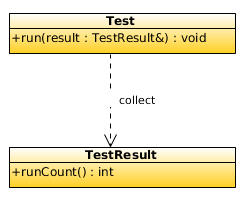
\includegraphics[width=0.4\textwidth]{figures/xunit/test-result.png}
\caption{聚集参数}
 \label{fig:test-result}
\end{figure}

糟糕的是,因为修改了抽象接口\ascii{Test::run}的函数签名信息,导致需要同步修改所有子类覆写\ascii{Test::run}的声明与实现,及其所有引用\ascii{Test::run}而导致编译失败的测试用例。这是\ascii{OO}设计固有的特质,因修改抽象接口的签名信息,连锁式地引发各个子类实现的修改。幸运的是,目前实现\ascii{Test}接口的所有子类都在可控的范围内,借助于编译器的提示,可以快速解决所有失败的编译问题。

最糟糕的情况是,接口对外已经发布稳定版本,存在大量外部客户的代码依赖。如果此后修改抽象接口的函数签名,将导致严重的兼容性问题。因此,对外发布抽象接口时,必须保持谨慎的态度。

\begin{nodiff}{include/mars/core/Test.h}
 \begin{c++}
#include <string>

@struct TestResult;@

struct Test {
  explicit Test(const std::string& = "");
  const std::string& getName() const;

  virtual void run(@TestResult&@) = 0;
  virtual ~Test() {}

private:
  std::string name;
};
 \end{c++}
\end{nodiff}

重构\ascii{TestCase::run}的声明与实现,增加聚集参数\ascii{TestResult}。

\begin{diff}{include/mars/core/TestCase.h, src/mars/core/TestCase.cc}
 \begin{minicpp}
#include <mars/core/Test.h>
#include <mars/core/TestFixture.h>

struct TestCase : Test, private TestFixture {
  using Test::Test;

private:
  void run(@TestResult&@) override;

private:
  virtual void runTest() {}
}
 \end{minicpp}
\tcblower
 \begin{minicpp}
#include <mars/core/TestCase.h>

void TestCase::run(@TestResult&@) {
  setUp();
  runTest();
  tearDown();
}
 \end{minicpp}
\end{diff}

重构\ascii{TestSuite::run}的声明与实现,增加聚集参数\ascii{TestResult}。实现\ascii{TestSuite::run}时,以引用的方式递归传递\ascii{TestResult}对象到各个子节点。此处,\ascii{TestResult}扮演聚集参数的角色,它顺延树结构的调用链传递,在每个调用关键节点处,收集、统计、诊断测试结果信息。

\begin{diff}{include/mars/core/TestSuite.h, src/mars/core/TestSuite.cc}
 \begin{minicpp}
#include <mars/core/Test.h>
#include <vector>

struct TestResult;

struct TestSuite : Test {
  using Test::Test;
  ~TestSuite();

  void add(Test* test);

private:
  void run(@TestResult&@) override;

private:
  template <typename F>
  void foreach(F f) const;

private:
  std::vector<Test*> tests;
};
 \end{minicpp}
\tcblower
 \begin{minicpp}
#include <mars/core/TestSuite.h>
#include <mars/core/TestCase.h>

void TestSuite::add(Test* test) {
  tests.push_back(test);
}

template <typename F>
inline void TestSuite::foreach(F f) const {
  for (auto test : tests) {
    f(test);
  }
}

TestSuite::~TestSuite() {
  foreach([](auto test) {
    delete test;
  });
}

void TestSuite::run(@TestResult& result@) {
  foreach([@&result@](auto test) {
    test->run(@result@);
  });
}
 \end{minicpp}
\end{diff}

为了关注于当前失败的测试用例,局部化修改其他编译失败的测试用例。可以局部性地引入\code{TestResult dummy},保证既有测试用例以最简单的方式通过,举例说明。

\begin{nodiff}{test/mars/core/TestMethodSpec.cc}
 \begin{c++}
#include <mars/core/TestMethod.h>
#include <mars/core/TestResult.h>
#include <gtest/gtest.h>

namespace {
  bool wasSucc;

  struct WasSucc : TestFixture {
    void testMethod() {
      wasSucc = true;
    }
  };

  struct TestMethodSpec : testing::Test {
  private:
    void SetUp() override {
      wasSucc = false;
    }

  protected:
    void run(::Test& test) {
      @TestResult dummy;@
      test.run(@dummy@);
    }
  };
}

TEST_F(TestMethodSpec, make_sure_test_running_is_succ) {
  TestMethod<WasSucc> test(&WasSucc::testMethod);

  ASSERT_FALSE(wasSucc);
  run(test);
  ASSERT_TRUE(wasSucc);
}
 \end{c++}
\end{nodiff}

至此,编译通过。

\subsubsection{通过测试}

为了尽快通过测试,伪实现\ascii{TestResult::runCount},直接返回\ascii{2}。

\begin{diff}{include/mars/core/TestResult.h, src/mars/core/TestResult.cc}
 \begin{minicpp}
struct TestResult {
  int runCount() const;
};
 \end{minicpp}
\tcblower
 \begin{minicpp}
#include <mars/core/TestResult.h>

int TestResult::runCount() const {
  return 2;
}
 \end{minicpp}
\end{diff}

通过测试。

\subsection{监听接口}

重构\ascii{TestResult}实现的伪代码,添加默认构造函数和监听接口\ascii{onStartTestCase},分别完成计数器的初始化和累加操作。

\begin{diff}{include/mars/core/TestResult.h, src/mars/core/TestResult.cc}
 \begin{minicpp}
struct TestResult {
  TestResult();

  void onStartTestCase();
  int runCount() const;

private:
  int numOfRuns;
};
 \end{minicpp}
\tcblower
 \begin{minicpp}
#include <mars/core/TestResult.h>

TestResult::TestResult() : numOfRuns(0) {
}

void TestResult::onStartTestCase() {
  numOfRuns++;
}

int TestResult::runCount() const {
  return numOfRuns;
}
 \end{minicpp}
\end{diff}

当\ascii{TestCase::run}被调用时,通知\ascii{TestResult}执行计数器累加操作。

\begin{nodiff}{src/mars/core/TestCase.cc}
 \begin{c++}
#include <mars/core/TestCase.h>
#include <mars/core/TestResult.h>

void TestCase::run(TestResult& result) {
@  result.startTestCase();@
  setUp();
  runTest();
  tearDown();
}
 \end{c++}
\end{nodiff}

此时,测试通过。提取子函数\ascii{TestCase::runBare},将监听器的调用逻辑与主干的算法逻辑相分离,突出主干逻辑的地位。

\begin{nodiff}{src/mars/core/TestCase.cc}
 \begin{c++}
#include <mars/core/TestCase.h>
#include <mars/core/TestResult.h>

void TestCase::runBare() {
  setUp();
  runTest();
  tearDown();
}

void TestCase::run(TestResult& result) {
  result.startTestCase();
  runBare();
}
 \end{c++}
\end{nodiff}

测试通过。

\end{content}

\section{统计器}

\begin{content}

\ascii{TestResult::runCount}在运行时,通过监听接口统计测试用例的数目。事实上,也可以遍历用例树,直接统计测试用例的数目。构造一个失败的用例,观察如何统计测试用例数目。

\subsection{抽象接口}

在\ascii{Test}增加抽象的查询接口\ascii{countTestCases},在运行时多态调用子类的相关实现。

\begin{nodiff}{test/mars/core/TestSuiteSpec.cc}
 \begin{c++}
#include <mars/core/TestSuite.h>
#include <mars/core/TestCase.h>
#include <gtest/gtest.h>

namespace {
  int countTestCases(Test& test) {
    return test.countTestCases();
  }
}

TEST(TestSuiteSpec, count_test_cases) {
  TestSuite suite;
  suite.add(new TestCase);
  suite.add(new TestCase);

  ASSERT_EQ(2, countTestCases(suite));
}
 \end{c++}
\end{nodiff}

\subsubsection{通过编译}

为了能够通过编译,在\ascii{Test}添加抽象接口\ascii{countTestCases}。

\begin{nodiff}{include/mars/core/Test.h}
 \begin{c++}
#include <string>

struct TestResult;

struct Test {
  explicit Test(const std::string& name = "");
  const std::string& getName() const;

  virtual ~Test() {}
@  virtual int countTestCases() const = 0;@
  virtual void run(TestResult&) = 0;

private:
  std::string name;
};
 \end{c++}
\end{nodiff}

在\ascii{TestCase}添加实现接口\ascii{countTestCases}。

\begin{nodiff}{include/mars/core/TestCase.h}
 \begin{c++}
#include <mars/core/Test.h>
#include <mars/core/TestFixture.h>

struct TestCase : Test, private TestFixture {
  using Test::Test;

private:
  void run(TestResult&) override;
@  int countTestCases() const override;@

private:
  virtual void runTest() {}

private:
  void runBare();
};
 \end{c++}
\end{nodiff}

在\ascii{TestSuite}添加实现接口\ascii{countTestCases}。

\begin{nodiff}{include/mars/core/TestSuite.h}
 \begin{c++}
#include <mars/core/Test.h>
#include <vector>

struct TestResult;

struct TestSuite : Test {
  using Test::Test;
  ~TestSuite();

  void add(Test* test);

private:
@  void run(TestResult& result) override;@
  int countTestCases() const override;

private:
  template <typename F>
  void foreach(F f) const;

private:
  std::vector<Test*> tests;
};
 \end{c++}
\end{nodiff}

至此,编译通过。

\subsubsection{通过测试}

通过测试也很简单,实现\ascii{TestCase::countTestCases}时,直接返回\ascii{1}。这不是伪实现,因为\ascii{TestCase}是叶子节点,返回常量\ascii{1}符合自身逻辑。

\begin{nodiff}{src/mars/core/TestCase.cc}
 \begin{c++}
int TestCase::countTestCases() const {
  return 1;
}
 \end{c++}
\end{nodiff}

实现\ascii{TestSuite::countTestCases}时,递归调用各个子节点的\ascii{countTestCases},完成累计操作。

\begin{nodiff}{src/mars/core/TestSuite.cc}
 \begin{c++}
int TestSuite::countTestCases() const {
  auto num = 0;
  foreach([&num](auto test) {
    num += test->countTestCases();
  });
  return num;
}
 \end{c++}
\end{nodiff}

至此,测试通过。

\subsection{函数式}

仔细观察\ascii{TestSuite}的成员函数\ascii{countTestCases},其实现逻辑本质上完成\ascii{reduce}操作。从\ascii{countTestCases}抽取更稳定的\ascii{reduce}函数,分离稳定与变化,高度复用代码逻辑。\ascii{reduce}复用\ascii{foreach},\ascii{countTestCases}复用\ascii{reduce}, 使其每个子函数关注变化的因素最小化。例如,\ascii{countTestCases}关心初始值,及其单元素的统计量。

\begin{nodiff}{src/mars/core/TestSuite.cc}
 \begin{c++}
template <typename F>
inline void TestSuite::foreach(F f) const {
  for (auto test : tests) {
    f(test);
  }
}

template <typename Init, typename F>
inline Init TestSuite::reduce(Init init, F f) const {
  foreach([&init, f](auto test) {
    init += f(test);
  });
  return init;
}

int TestSuite::countTestCases() const {
  return reduce(0, [](auto test){
    return test->countTestCases();
  });
}
 \end{c++}
\end{nodiff}

事实上,\ascii{C++98}已经具备完备的函数式编程能力,包括函数指针,函数对象。只是设计与实现\emph{函数对象}时,捕获上下文信息并不容易,容易产生重复代码。借助于\ascii{C++11}的\ascii{lambda}表达式,闭包能力得到完全释放,实现变得极其简单。

\ascii{C++11}的\ascii{lambda}表达式附加\emph{捕获列表},方便用户根据场景灵活定制。\cpp{}始终秉承自由的哲学观,致力寻找抽象与性能之间的平衡点。相反,相对大部分编程语言实现\ascii{lambda}表达式时,默认地捕获整个上下文,在内存与性能方面\cpp{}优势非常明显。

\end{content}
